\chapter{Figures and Visualizations}
\label{ch:figures}

This chapter compiles key visualizations that support the ESQET framework and its predictions, generated either through simulations or conceptual diagrams.

\section{Conceptual Wormhole Diagram with Fibonacci Spiral}
This diagram conceptually illustrates an Einstein-Rosen bridge (wormhole) where the Golden Ratio ($\phiGolden$) and Fibonacci patterns are crucial for stabilizing its throat. The Fibonacci spiral symbolizes how $\phiGolden$-scaled entanglement might provide the necessary coherent structure for traversable wormholes.

\begin{figure}[h!]
    \centering
    % LaTeX/TikZ code for Conceptual Wormhole Diagram
    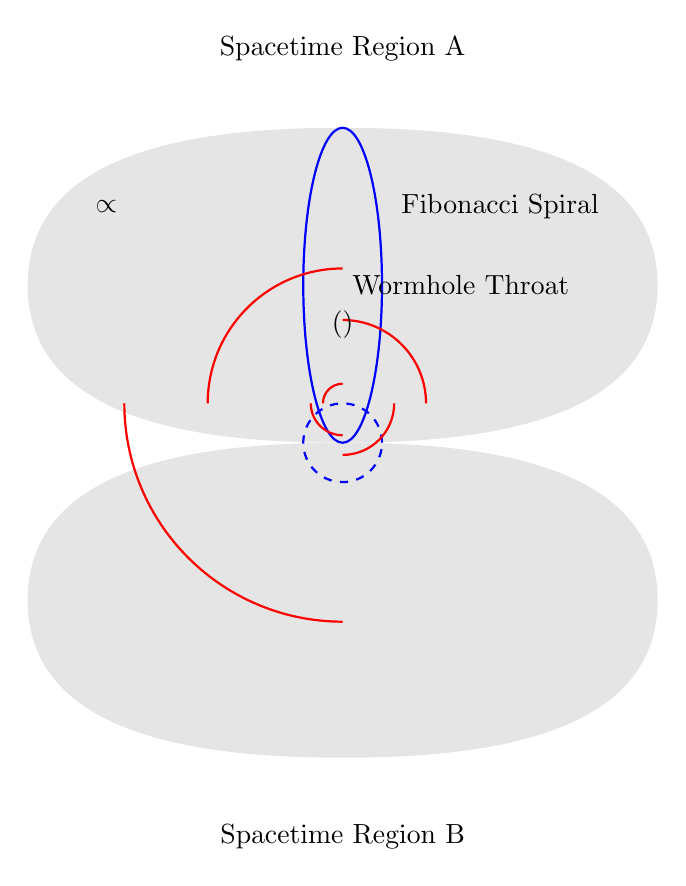
\begin{tikzpicture}
        % Spacetime sheets
        \fill[gray!20] (-4,0) to[out=90,in=180] (0,2) to[out=0,in=90] (4,0) to[out=270,in=0] (0,-2) to[out=180,in=270] (-4,0);
        \fill[gray!20] (-4,-4) to[out=90,in=180] (0,-2) to[out=0,in=90] (4,-4) to[out=270,in=0] (0,-6) to[out=180,in=270] (-4,-4);

        % Wormhole throat
        \draw[thick, blue] (0,0) ellipse (0.5cm and 2cm);
        \draw[thick, blue, dashed] (0,-2) ellipse (0.5cm and 0.5cm);

        % Fibonacci spiral - adjusted for visual effect and simplicity
        % You might need to tweak r and center to align perfectly
        \def\phi{1.6180339887} % More precise phi
        \def\rStart{0.25} % Starting radius for the spiral
        \def\spiralCenter{(0, -1.5)} % Center point for the spiral near the throat

        \foreach \i in {0,1,2,3,4,5} { % Drawing segments of the spiral
            \draw[red, thick] \spiralCenter ++({90+\i*90}:\rStart*\phi^\i) arc ({90+\i*90}:{180+\i*90}:\rStart*\phi^\i);
        }

        % Annotations
        \node at (-3,1) {$\Dent \propto \phiGolden$};
        \node at (3,-5) {$\rhoExotic$};
        \node at (0,3) {Spacetime Region A};
        \node at (0,-7) {Spacetime Region B};
        \node at (1.5,0) {Wormhole Throat};
        \node at (2,1) {Fibonacci Spiral};
        \node at (0,-0.5) {$\FQC(\phiGolden)$}; % Emphasize FQC's role
    \end{tikzpicture}
    \caption{Conceptual diagram of an Einstein-Rosen Bridge (Wormhole) stabilized by $\phiGolden$-scaled entanglement, visualized through a Fibonacci spiral representing coherent spacetime structure.}
0
    \label{fig:wormhole_fibonacci}
\end{figure}

\section{Simulation Visualizations}
This section will contain the plots generated by the Python simulations, providing visual evidence of the ESQET framework's behavior.

\begin{figure}[h!]
    \centering
    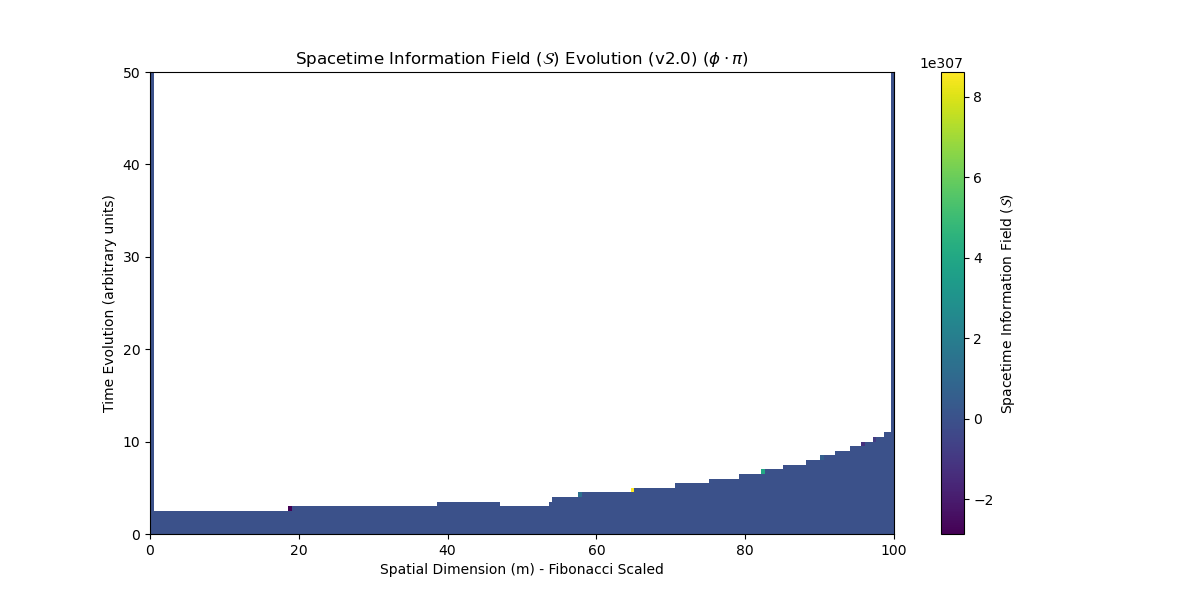
\includegraphics[width=0.8\textwidth]{figures/fibonacci_spacetime_evolution_v2.png} % <-- UPDATED FILENAME
    \caption{Heatmap of the Spacetime Information Field ($\Sfield$) evolution on a Fibonacci-scaled spatial grid. (Generated by `fibonacci_spacetime_evolution_sim.py`)}
    \label{fig:s_evolution_v2}
\end{figure}

\begin{figure}[h!]
    \centering
    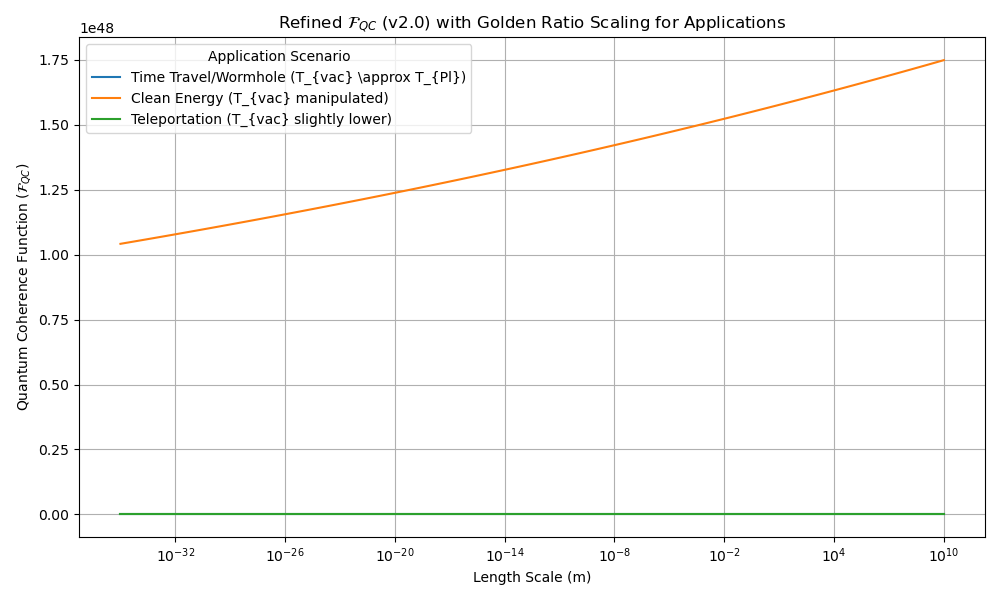
\includegraphics[width=0.8\textwidth]{figures/fibonacci_F_QC_applications_v2.png} % <-- UPDATED FILENAME
    \caption{The Quantum Coherence Function ($\FQC$) across length scales for different application scenarios, with $\phiGolden$ scaling. (Generated by `fibonacci_F_QC_applications_sim.py`)}
    \label{fig:fqc_applications_v2}
\end{figure}

